\documentclass[a4paper,10pt]{article}
\usepackage[T1]{fontenc}
\usepackage{lmodern,microtype,amsmath,amssymb,graphicx,booktabs,tabularx}
\usepackage[section]{placeins}
\usepackage[textwidth=7.16in,top=18mm,bottom=18mm]{geometry}
\usepackage[font=small,labelfont=bf]{caption}
\usepackage[colorlinks=true,linkcolor=blue,urlcolor=blue,citecolor=blue]{hyperref}
\hypersetup{pdftitle={When Background Noise Has Meaning: Research Report},pdfauthor={Qihan Zhu}}
\setlength{\parindent}{0pt}
\setlength{\parskip}{5pt plus 1pt}
\setlength{\textfloatsep}{12pt}
\renewcommand{\topfraction}{0.95}
\renewcommand{\bottomfraction}{0.95}
\renewcommand{\textfraction}{0.05}
\renewcommand{\floatpagefraction}{0.7}
\newcommand{\corefig}[3]{\begin{figure}[tbp]\centering\includegraphics{../results/report_figure_assets_20261109/#1.pdf}\caption{#2}\label{#3}\end{figure}}
\newcommand{\diagfig}[3]{\begin{figure}[tbp]\centering\includegraphics{../results/extensions_20261109/figures/#1.pdf}\caption{#2}\label{#3}\end{figure}}
\newcommand{\closingfig}[3]{\begin{figure}[tbp]\centering\includegraphics{../results/closing_20261110/figures/#1.pdf}\caption{#2}\label{#3}\end{figure}}
\begin{document}
\begin{center}
{\LARGE\bfseries When Background Noise Has Meaning}\\[4pt]
{\Large Environmental Sound Classification under Semantic Interference}\\[7pt]
Qihan Zhu \quad SID 550489593 \quad ELEC5305\\[3pt]
Research report draft --- closing analyses and review 10 November 2026
\end{center}

\begin{abstract}
Environmental recordings often contain more than one recognisable event. This
study compares a handcrafted 92-feature SVM, a compact log-Mel CNN and frozen
zero-shot LAION-CLAP on all five official ESC-50 folds. Identical white-noise,
DEMAND-background and labelled event mixtures are tested at +10, +5 and 0 dB,
with gain-matched controls and two activity-based power definitions. The SVM is
especially vulnerable to white noise; CLAP retains stronger generic-background
performance while frequently predicting a competing event. Temporal overlap
changes the CNN comparison, and its negative semantic-minus-DEMAND contrast
replicates directionally across three training seeds. In the expanded experiment,
WGN augmentation raises three-seed CNN macro-F1 under +5-dB white noise from
7.48\% to 43.95\%, but changes same-category semantic performance only from
32.99\% to 33.46\%. Semantic augmentation reaches 36.05\% in that condition,
while clean macro-F1 falls from 65.78\% to 61.70\%; its modest direct CNN
advantages over WGN training do not pass the declared multiplicity correction.
A fixed prompt ensemble raises CLAP clean accuracy from 81.75\% to 92.90\%
without changing audio embeddings, yet a substantial semantic-interference gap
remains. Capture destinations, full-class rankings and within-model feature
shifts expose failure structure that aggregate accuracy misses. At +5 dB,
one-third of single-template CLAP captures retain the target at rank two.
On small subsets matched closely on measured spectral and temporal proxies,
CLAP retains a semantic-minus-DEMAND accuracy disadvantage while CNN intervals
include zero; selection and unmeasured acoustics limit this interpretation. The contribution
is a reproducible DSP experiment with measured robustness trade-offs, rather
than an equal-data model contest or causal isolation of meaning from acoustics.
\end{abstract}

\section{Research question and context}
A single-label environmental-sound benchmark usually identifies a dominant
event. Deployment audio can contain a dog bark and an alarm simultaneously.
Equal interference power does not imply equal spectral structure, temporal
overlap, recognisability or perceptual prominence. The main question is therefore:
\emph{How do different audio representations fail under ordinary acoustic noise
and a competing meaningful event at controlled relative levels?} Two further
questions ask whether an error identifies the distractor and whether ordinary
noise augmentation transfers to competing meaningful events.

ESC-50 provides a small balanced benchmark with official folds
\cite{esc,esc_repo}. Spectrogram CNNs established a learned alternative to
handcrafted descriptors \cite{piczak_cnn}; augmentation has also been studied
for environmental-sound classification \cite{augmentation}. A third paradigm,
contrastive audio-language pretraining, permits classification through similarity
to textual class descriptions \cite{clap}. These systems have very different
external training histories. Their comparison here concerns deployment behaviour,
not equal-data training efficiency.

Recent work motivates a closer examination of structured interference. PAT
uses training-free cross-modal alignment and evaluates noisy inputs
\cite{pat}. Mix-CLAP studies noise-aware audio-language models and efficiency
\cite{mixclap}. RSA-Bench constructs complex acoustic backgrounds for speech
perception and reasoning tasks \cite{rsa}. That benchmark is related motivation,
not a direct environmental-event classification baseline. This project does not
reproduce those model-training programmes.

\section{Dataset, models and validation}
\subsection{Official folds and data handling}
ESC-50 contains 2,000 five-second recordings, 50 balanced classes and five
predefined folds. All 50 classes are retained. For outer fold $k$, fold
$(k\bmod 5)+1$ supplies validation data and the remaining three folds supply
selection training data. After selecting hyperparameters or training duration,
a fresh model is fitted on the four non-test folds. Test labels are used only
for evaluation. Feature standardisation and Mel normalisation are estimated
from the applicable training partition.

The data audit identifies four source IDs spanning official folds, affecting
nine target clips. Official assignments are preserved and documented; those
sources are excluded from semantic-distractor eligibility. Consequently, the
experiment should not be described as perfectly source-independent. The
dataset authors also document partly class-dependent preprocessing
\cite{esc_repo}; clean benchmark performance is not evidence of unrestricted
real-world generalisation.

\subsection{DSP and classical baseline}
The custom STFT uses a 1,024-sample periodic Hann window, a 512-sample hop and a
1,024-point FFT at 44.1 kHz. Frames start at sample zero; only the final incomplete
frame is zero-padded. The output contains 513 complex one-sided bins. No
per-clip amplitude normalisation or pre-emphasis is applied. Agreement is checked
against SciPy and against an actual MATLAB execution of the unmodified course
\texttt{MyStft.m}. The latter comparison explicitly reconciles the supplied
window, leading padding, frame offsets and full/one-sided spectra. On a real
ESC-50 recording the relative complex-valued error is approximately
$2.6\times10^{-16}$. This verifies corresponding frames, not identical boundary
policies or default window helpers.

The handcrafted representation aggregates means and standard deviations of
RMS, zero-crossing rate, spectral centroid, spread, roll-off, flux, 20 MFCCs and
their deltas, giving 92 dimensions. An RBF SVM uses training-only standardisation.
The original nine-candidate grid combines $C\in\{1,10,100\}$ with
$\gamma\in\{\texttt{scale},0.001,0.1\}$, selected by clean validation macro-F1.
The implementation retains one-vs-rest decision scores and explicit tie handling.

\subsection{Compact CNN and frozen CLAP}
The CNN uses 64 Mel bands, log compression, and three convolution/normalisation/
ReLU/pooling blocks with 16, 32 and 64 channels. Temporal pooling and four
frequency bins yield a 256-dimensional representation before the classifier.
It has 36,258 trainable parameters. Adam uses learning rate $10^{-3}$, weight decay
$10^{-4}$, batch size 32 and dropout 0.3. Training is capped at 40 epochs with
patience 8; clean validation selects duration before a fresh four-fold refit.
The core experiment uses seed 5305. Additional seeds are analysed separately.

CLAP uses the fixed \texttt{630k-audioset-best.pt} checkpoint, HTSAT-tiny audio
encoder, RoBERTa text encoder and no fusion. Audio is resampled to 48 kHz and
passes through the official int16 truncation-and-return convention exactly once.
That conversion clips to $[-1,1]$ after resampling. The mixer's no-hard-clipping
guarantee concerns the canonical input waveform before model-specific preprocessing.
The official non-fusion frontend repeat-pads five-second inputs to ten seconds;
all systems receive the same canonical five-second waveform before their own
frontends.
The prompt is \texttt{the sound of \{label\}}, replacing underscores with spaces.
Class scores are cosine similarities between unit audio embeddings and the 50
unit prompt embeddings. Parameters are frozen; there is no ESC-50 classifier
training, prompt selection or fine-tuning. Checkpoint SHA-256 starts
\texttt{8053c977}; the complete hash is stored with the results. External
pretraining overlap cannot be ruled out merely because inference is zero-shot.

\section{Controlled interference and the power-definition change}
Each target receives white Gaussian noise, a five-second segment from one of
three DEMAND recordings (traffic, station and metro) \cite{demand}, one same-coarse-category
ESC-50 distractor and one different-coarse-category distractor. Semantic
distractors have a different fine class and source recording and come from the
target's held-out fold. Pairing is deterministic. Within each target/condition,
the exact noise waveform, DEMAND segment or semantic pair is fixed across the
three levels. Semantic events use zero relative offset.
DEMAND is a real-background control, not a guarantee of semantically empty
audio: traffic or station recordings can contain recognisable events. The
semantic-distractor condition adds a known competing ESC-50 class, enabling
label-specific capture analysis; it does not isolate meaning from every acoustic
difference between conditions.

Let $x[n]$ be the target and $d[n]$ the interferer. Activity masks contain samples
covered by unwindowed frames whose mean-square energy is within 40 dB of the
corresponding peak frame. Define $P(z;M)=|M|^{-1}\sum_{n\in M}z[n]^2$.
For requested level $L$,
\begin{align}
P_x &=P(x;M_x),\\
P_d^{\mathrm{own}}&=P(d;M_d),\qquad
P_d^{\mathrm{target}}=P(d;M_x),\\
\alpha&=\sqrt{P_x/(10^{L/10}P_d)},\qquad
y[n]=g\bigl(x[n]+\alpha d[n]\bigr),\\
g&=\min\!\left(1,\frac{0.99}{\max_n|x[n]+\alpha d[n]|}\right).
\end{align}
The matching clean control is $gx[n]$. Common attenuation preserves the
component-power ratio and avoids hard clipping. Achieved ratios are recomputed
numerically rather than assumed from the gain formula.

\textbf{Deviation from the proposal.} The proposal specified the target-mask
definition. In preliminary implementation, sparse distractors with little
energy inside $M_x$ required very large gains, even when their event occurred
outside the target-active interval. The default was therefore changed to
own-activity power. The originally proposed target-mask protocol was also run
in full as a sensitivity analysis. The two ratios answer different measurement
questions; neither is an automatic correction for temporal overlap, and the
choice is not attributed to an unrecorded instructor instruction.

There are 24,000 own-protocol mixtures. Three target/distractor pairs have zero
interferer energy on the target mask; their three levels are undefined under
the target protocol and are excluded with recorded reasons, leaving 23,991
mixtures. Cross-protocol comparisons use common retained targets. The manifest
records target/distractor identity, labels, categories, folds, hashes, seeds,
offsets, gains, both measured power ratios, peak control and activity overlap
$|M_x\cap M_d|/|M_x|$. The 0-dB condition is a deliberately ambiguous
single-label stress test, not an ordinary equal-difficulty accuracy benchmark.

\section{Outcomes and statistical treatment}
Accuracy and macro-F1 are computed within each official test fold, with means
and sample standard deviations across five folds. Macro-F1 retains all 50 class
labels. For a semantic condition, distractor capture rate is the number of wrong
predictions equal to the distractor divided by the number of errors. The
unconditional capture fraction uses all trials instead. A reference of $1/49$
assumes uniform choice among wrong labels; it is not an empirical null for
class-dependent confusion.

The target--distractor margin subtracts the distractor score from the target
score. Scores are SVM decision values, CNN logits or CLAP cosines and are
interpreted only within a system. A negative margin does not guarantee that
the distractor beats every other class. The CLAP diagnostic therefore also
computes ranks and competing scores across all 50 prompts.

Relative macro-F1 loss is $1-F_{\mathrm{mixture}}/F_{\mathrm{clean}}$, where each
$F$ is the five-fold mean on identical retained targets. It is a proportional
loss, not a percentage-point difference. Replacing the reference with
$F_{\mathrm{gain\ control}}$ gives the additional control-referenced loss.
Capture rates pool counts across folds; they are not unweighted means of fold
capture percentages. Fold SD describes between-fold variation, not a confidence
interval for a population mean.

Paired bootstrap intervals resample target clips within official folds,
retaining matched condition predictions, using 2,000 replicates and seed 530509.
For these matched comparisons, accuracy differences pool the retained target
trials; macro-F1 differences average the fold-specific values.
They condition on the fitted models and do not incorporate refitting or all
source-recording dependence. Exact McNemar comparisons use paired correctness.
Holm correction covers the 12 +5-dB high-overlap comparisons across models,
power definitions and semantic pairing types. These are post-baseline extensions,
not retrospectively preregistered tests. Three CNN seeds separately assess
training variability; five folds times three seeds are not 15 independent datasets.

Three comparison families are kept distinct: 12 core high-overlap contrasts
(three systems, two power protocols and two semantic pairing types); 12 clean-CNN
replication contrasts (three seeds, two protocols and two pairing types); and 156
intervention contrasts, defined in the extension protocol. A core seed-5305
comparison appears in both of the first two families, so its adjusted $p$ value
can differ without its effect or raw $p$ value changing. Holm correction applies
within each family; it is not a study-wide guarantee across every exploratory
analysis. Bootstrap intervals are pointwise and unadjusted. Exact McNemar tests
assume independent target pairs under the null; shared source recordings,
distractors, backgrounds and overlapping training sets limit that assumption.
The corrected values therefore remain conditional, nominal tests, rather than
proof of generalisation to independently sampled acoustic scenes.

An exploratory resampling-unit sensitivity analysis draws 10,000 bootstrap
samples of original target source IDs globally. All retained clips from a sampled
source move together, including the rare source spanning official folds. It
estimates the pooled matched-target accuracy difference. These pointwise source-
cluster intervals condition on fitted models, do not replace the declared Holm
families, and do not capture every dependency from shared distractors or backgrounds.

\section{Core results}
\begin{table}[htbp]\centering
\caption{Clean five-fold results (percent; mean $\pm$ sample SD). Core CNN seed: 5305.}
\label{tab:clean}\begin{tabular}{lrr}\toprule System & Accuracy & Macro-F1\\\midrule
SVM & 48.90 $\pm$ 4.21 & 47.96 $\pm$ 4.07 \\
CNN & 67.90 $\pm$ 3.65 & 66.61 $\pm$ 3.91 \\
CLAP & 81.75 $\pm$ 2.58 & 79.49 $\pm$ 3.28 \\\bottomrule\end{tabular}\end{table}
\begin{table}[htbp]\centering
\caption{Macro-F1 at +5 dB (percent; five-fold mean $\pm$ sample SD). Each cell uses its retained targets.}
\label{tab:five}\begin{tabular}{llrrr}\toprule Power & Condition & SVM & CNN & CLAP\\\midrule
Own & White noise & 2.03 $\pm$ 0.86 & 7.76 $\pm$ 1.54 & 62.91 $\pm$ 3.50 \\
Own & DEMAND & 16.13 $\pm$ 1.95 & 29.46 $\pm$ 4.19 & 71.49 $\pm$ 1.00 \\
Own & Same category & 22.47 $\pm$ 2.68 & 32.60 $\pm$ 2.26 & 48.86 $\pm$ 1.53 \\
Own & Different category & 21.34 $\pm$ 2.58 & 32.00 $\pm$ 3.38 & 45.16 $\pm$ 1.11 \\
\midrule
Target & White noise & 2.03 $\pm$ 0.86 & 7.76 $\pm$ 1.54 & 62.92 $\pm$ 3.50 \\
Target & DEMAND & 16.15 $\pm$ 2.29 & 29.33 $\pm$ 4.14 & 71.64 $\pm$ 0.91 \\
Target & Same category & 21.14 $\pm$ 2.63 & 31.70 $\pm$ 1.88 & 47.76 $\pm$ 1.07 \\
Target & Different category & 20.87 $\pm$ 2.37 & 30.93 $\pm$ 4.19 & 42.81 $\pm$ 1.27 \\
\bottomrule\end{tabular}\end{table}

Table~\ref{tab:clean} establishes the three clean reference points. Table~\ref{tab:five}
shows +5-dB macro-F1 for each power definition; the complete level curves are
in Figure~\ref{fig:robustness}. The SVM is severely affected by white noise,
whereas meaningful distractors are less damaging in its aggregate results.
This contradicts a universal assertion that semantic interference must always
be harder than generic noise. CLAP is comparatively robust to ordinary
backgrounds but experiences a much larger semantic-interference penalty.

\corefig{fig1_macro_f1_vs_level}{Core robustness curves under own-activity power. Values are five-fold macro-F1 means; error bars are sample SD, not confidence intervals. The same input mixtures are used by all systems. Zero dB is the equal-power stress test.}{fig:robustness}

Under the own protocol at +5 dB, CLAP's capture rates are approximately 67\%
for same-category and 60\% for different-category distractors. The corresponding
CNN values are about 31\% and 28\%, and SVM values about 19\% and 16\%.
These are fractions of errors, not percentages of all targets. Capture and
margin curves describe increasingly strong distractor competition as SIR falls
(Figures~\ref{fig:capture} and \ref{fig:margin}). Both absolute accuracy and
capture denominators must accompany this interpretation.

\corefig{fig2_capture_rate_vs_sir}{Distractor capture among incorrect trials. The horizontal reference is uniform wrong-label choice, not a class-conditioned null distribution. Same-category and different-category pairings are distinguished by line style.}{fig:capture}

\subsection{Overlap and matched comparisons}
The whole-dataset CNN ranking between semantic interference and DEMAND is
affected by the composition of low-overlap mixtures. Compare each semantic
condition against DEMAND on precisely the same targets, stratified by overlap.
At overlap at least 0.8 and +5 dB, CNN semantic accuracy is about three percentage
points lower. Pointwise paired bootstrap intervals exclude zero, but the
Holm-adjusted exact McNemar p-values are approximately 0.12--0.15. The appropriate
claim is a consistent observed direction requiring replication, rather than
an established family-wise significant CNN effect.

CLAP's corresponding losses are much larger: own-protocol differences are
-25.55 points (same category) and -28.53 points (different category), with paired
95\% intervals [-28.28,-22.95] and [-31.20,-25.73]. The target protocol gives
similarly large differences. Figure~\ref{fig:paired} separates these effects
from the small, uncertain SVM differences. Stratified macro-F1 is also reported,
but it can be depressed by missing classes; matched accuracy and class coverage
are used to interpret stratum difficulty.

\diagfig{09_paired_accuracy_intervals}{Semantic-minus-DEMAND accuracy on matched high-overlap targets at +5 dB. Intervals are 2,000-replicate paired target-level bootstrap intervals within folds, conditional on the trained models. They are pointwise intervals; the text separately reports multiplicity-adjusted tests.}{fig:paired}

Changing power convention moderately lowers semantic performance but does not
remove the main model-specific pattern. It should not be claimed that every
fine ranking is invariant: small same-/different-category order changes can
occur, including for the CNN at 0 dB. Both protocols and the retained-target
intersection remain part of the result rather than selecting a preferred table.

\subsection{Gain-matched control check}
Table~\ref{tab:gain} compares attenuated and original clean audio on matched
targets. The shifts are small relative to mixture losses, but are not zero.
\begin{table}[htbp]\centering\small
\caption{Gain-matched clean minus original clean macro-F1 at +5 dB, in percentage points. Each value is a difference of five-fold means on that condition's retained targets. Core CNN seed: 5305.}
\label{tab:gain}\begin{tabular}{llrrrr}\toprule Power & Model & White & DEMAND & Same & Different\\\midrule
Own & SVM & -0.25 & -0.19 & -0.64 & -0.76 \\
Own & CNN & +0.28 & +0.25 & -0.10 & +0.03 \\
Own & CLAP & +0.25 & +0.15 & +0.11 & +0.45 \\
\midrule
Target & SVM & -0.25 & -0.22 & -0.47 & -0.48 \\
Target & CNN & +0.28 & +0.25 & -0.35 & -0.32 \\
Target & CLAP & +0.25 & +0.15 & +0.40 & +0.13 \\
\bottomrule\end{tabular}\end{table}
Across all 72 core cells, control-minus-clean F1 ranges from -1.74 to +0.49 percentage points. Both reference losses are exported; these results show limited attenuation effects, not exact amplitude invariance.


\section{Representation and competition diagnostics}
Handcrafted displacement uses the relevant SVM training-fold scale and is
normalised by the square root of group dimensionality. The eight groups are
RMS, ZCR, centroid, spread, roll-off, flux, MFCCs and delta-MFCCs. At +5 dB,
white noise shifts ZCR and spectral shape descriptors far more than the other
conditions (Figure~\ref{fig:groups}). This offers a concrete DSP explanation
for the SVM's extreme white-noise sensitivity without treating feature movement
as sufficient to explain every wrong label.

\diagfig{10_feature_group_displacement}{Median clean-control-to-mixture displacement for eight handcrafted feature groups at +5 dB. Each group uses training-fold standardisation and division by the square root of its dimension. The shared logarithmic colour scale is a display scale; annotated values are untransformed distances.}{fig:groups}

CNN and CLAP movement uses cosine distance between mixture and gain-matched
clean embeddings. Distances are not compared absolutely across architectures.
For high-overlap CNN pairs, semantic interference can produce worse accuracy
despite smaller movement than matched DEMAND backgrounds. This is compatible
with direction-sensitive decision boundaries, but does not prove that semantic
meaning itself caused the effect. CLAP behaves differently: its high-overlap
semantic mixtures generally move farther than the matched DEMAND embeddings.

CLAP also exposes the destination of movement. Under own-activity power,
the same-category distractor's median rank improves from 17 in the clean control
to 4, 3 and 2 at +10, +5 and 0 dB. Figure~\ref{fig:ranks} shows the complete
50-class ranking diagnostic. Scores for the three highest other competing
classes are retained per trial. Displacement/error AUC (Appendix) summarises
association within each condition and fold, not causal explanation.

\diagfig{11_clap_distractor_ranking}{CLAP distractor ranking among all 50 classes. Lower rank is stronger; rank 1 is highest. Top-five fractions use all semantic trials, unlike error-conditioned capture rate. Grey curves are gain-matched clean controls.}{fig:ranks}

\subsection{The remaining competing classes}
An error need not name the designated distractor. For each CLAP mixture, define
$o^*=\arg\max_{c\notin\{x,d\}}s_c$ over the other 48 labels.
Table~\ref{tab:other} retains all three possible prediction destinations and
shows the target's margin over this strongest other class. The last column
subtracts that same class's gain-matched control score from its mixture score.
Because $o^*$ is selected on the mixture, this is a descriptive selected-competitor
diagnostic; it is not evidence for a prespecified class effect.
\begin{table}[htbp]\centering\footnotesize
\caption{Single-prompt CLAP at +5 dB. Target, distractor and other columns are disjoint prediction counts summing to $n$. The final two columns are median cosine-score differences, not probabilities.}
\label{tab:other}\begin{tabular}{llrrrrrr}\toprule Power & Pair & $n$ & Target & Distractor & Other & $s_x-s_{o^*}$ & $\Delta s_{o^*}$\\\midrule
Own & Same & 2000 & 1056 & 632 & 312 & +0.062 & +0.047 \\
Own & Different & 2000 & 985 & 612 & 403 & +0.044 & +0.055 \\
Target & Same & 1998 & 1032 & 664 & 302 & +0.057 & +0.053 \\
Target & Different & 1999 & 943 & 647 & 409 & +0.036 & +0.062 \\
\bottomrule\end{tabular}\end{table}

\subsection{Closing analysis: a ranked two-label readout}
These final analyses use existing predictions and audio only. They are exploratory:
the protocol was fixed after inspecting the cloud top-two and partial acoustic
results, before the local DEMAND completion. No model, prompt or dataset was
added. The original single-label results remain unchanged.

An argmax capture does not establish that the target has disappeared from the
ranking. We therefore select exactly the top $k$ labels, with $k=2$ primary and
$k\in\{1,3,5\}$ as sensitivity checks. Equal scores use ascending class ID; no
ties occurred at the inspected boundaries. Both the target and distractor ranks
are recovered from all 50 saved scores, including gain-matched clean controls.
For each designated pair the four states are target only, both, distractor only
and neither. Fractions use all semantic trials, whereas target retention among
captures conditions on the original prediction equalling the distractor.
There are 23,991 semantic trials per system or text-readout variant across both
power definitions. This is ranked retrieval, not a calibrated multi-label
detector: two labels are always returned, and a rank does not demonstrate
subjective hearing or complete source recovery.

\begin{table}[htbp]\centering\small
\caption{CLAP top-two states at +5 dB (percent of all semantic trials). Last column: target in top two among original argmax captures, a different denominator. Own uses 2,000 targets per type; target uses 1,998 same-category and 1,999 different-category targets.}
\label{tab:top2}\begin{tabular}{lllrrrrr}\toprule
Power & Text readout & Type & Target only & Both & Distractor only & Neither & Retained\\\midrule
Own & Single & Same & 43.95 & 26.05 & 23.35 & 6.65 & 37.34 \\
Own & Single & Different & 44.60 & 21.00 & 24.05 & 10.35 & 33.17 \\
Own & Ensemble & Same & 41.55 & 36.65 & 19.05 & 2.75 & 47.60 \\
Own & Ensemble & Different & 45.55 & 28.45 & 22.90 & 3.10 & 38.60 \\
\midrule
Target & Single & Same & 42.09 & 26.73 & 24.72 & 6.46 & 36.45 \\
Target & Single & Different & 41.97 & 22.16 & 25.66 & 10.21 & 32.92 \\
Target & Ensemble & Same & 38.99 & 38.34 & 19.92 & 2.75 & 47.85 \\
Target & Ensemble & Different & 42.47 & 29.96 & 24.41 & 3.15 & 38.65 \\
\bottomrule\end{tabular}\end{table}

At +5 dB under own power, the single-template target remains second in
236/632 same-category captures (37.34\%) and 203/612 different-category captures
(33.17\%). Joint top-two inclusion occurs in 26.05\% and 21.00\% of all mixtures,
compared with 5.40\% and 1.70\% of their clean controls. Yet 23.35\% and 24.05\%
contain only the distractor among the two designated labels. The existing prompt
ensemble retains the target in 47.60\% and 38.60\% of captures. The target-power
analysis gives a similar partial recovery (Table~\ref{tab:top2}). Thus some
single-label failures retain useful target ranking, while the top-two readout
does not remove the interference problem. Increasing $k$ mechanically makes
inclusion easier; Figure~\ref{fig:retention} reports that trade-off without
reclassifying the original errors as correct. Even the two designated source
labels need not exhaust every audible event in a recording.

\closingfig{20_readout_top2_single}{Exact top-two states for frozen single-template CLAP. Each SIR has gain-matched control (left) and mixture (right). Four states partition every designated target--distractor pair; the states are not perceptual detection claims. Counts and all-system sensitivities accompany the figure.}{fig:top2}

\subsection{Closing analysis: spectral and temporal overlap}
All 24,000 own-power and 23,991 target-power rows now have acoustic descriptors,
including 6,000 DEMAND rows in each protocol. The legacy long-term dB Mel
correlation, linear spectral cosine, target time--frequency masking fraction,
energy-weighted masking fraction and temporal activity overlap are retained.
We add a cosine between spectra averaged only over target-active frames and a
dB correlation after dividing each Mel band by its summed filter weights.
The latter is a bandwidth-normalised density diagnostic. All use the project's
64-band DSP/CNN frontend, not CLAP's internal frontend. A target-active frame
has unwindowed energy within 40 dB of its peak; a target-active time--frequency
cell is within 40 dB of peak Mel-cell power. The masked-cell fraction counts
those cells where scaled interference power exceeds target power. It is a
computational proxy, not a validated measure of perceptual masking. Undefined
target-active cosines are left missing (nine own-power rows), not replaced by zero.

This frontend detail changes the interpretation of the preliminary analysis.
At +5 dB the white-noise median raw dB Mel correlation is $-0.728$; after
bandwidth normalisation it is $-0.008$ (Figure~\ref{fig:acoustic-distributions}).
White-noise power per unequal-width Mel band is not flat, even when its power
density is flat. The apparent anticorrelation is therefore not evidence that
white noise physically avoids the target spectrum. Median masked-cell fractions
are 0.319 for white noise, 0.146 for DEMAND, 0.121 for same-category events and
0.120 for different-category events under own power. These marginal summaries
describe different spectral and temporal structures, not equivalent acoustic
difficulty or semantic causality.

\closingfig{22_acoustic_distributions_own}{Acoustic descriptor distributions at +5 dB, own-power protocol. Each box represents 2,000 target mixtures; whiskers extend to 1.5 interquartile ranges. Bandwidth normalisation changes the white-noise correlation interpretation. Masking is a time--frequency proxy; each descriptor has its own scale. Target-power distributions are exported separately.}{fig:acoustic-distributions}

\FloatBarrier
\subsection{Same-target comparisons with close acoustic descriptors}
The primary +5-dB comparison retains a target only when its two mixtures differ
by at most 0.10 in target-active spectral cosine, 0.05 in masked-cell fraction,
and 0.10 in temporal overlap. Selection uses audio descriptors alone and is
identical for SVM, core CNN seed 5305 and single-template CLAP. Strict
$(0.05,0.025,0.05)$ and loose $(0.20,0.10,0.20)$ versions accompany it, as do
all-target and high-temporal-overlap comparisons. These calipers improve
agreement on measured descriptors; they do not make the waveforms identical.

The primary same-/different-category versus DEMAND subsets retain 210/178
targets under own power (199/168 source clusters; 49/48 classes) and 205/187
under target power (195/178 clusters; 49/47 classes). Only about 9--10.5\% of
the benchmark is retained. Accuracy differences compare the same targets within
each selected subset. Pointwise 95\% percentile intervals use 2,000 bootstrap
resamples of original target-recording IDs, keeping clips from one source
together (seed 530510). They are conditional on the fitted models and observed
pairings; shared interferers, backgrounds and training-set dependence are not
fully captured. No new family of significance tests is introduced. Intervals
are omitted when either target or source-cluster count is below 30.

\begin{table}[htbp]\centering\small
\caption{Accuracy difference in the primary acoustic-closeness subsets at +5 dB: semantic minus DEMAND, percentage points [pointwise 95\% source-bootstrap interval]. Positive favours the semantic mixture. Each column compares identical targets within its own subset; subset sizes are given in the text.}
\label{tab:acoustic-matched}\begin{tabular}{llrr}\toprule
Power & Model & Same category minus DEMAND & Different category minus DEMAND\\\midrule
Own & SVM & +1.90 [-4.42, +8.13] & +8.43 [+2.78, +14.61] \\
Own & CNN & +3.81 [-3.33, +11.79] & +2.25 [-3.37, +7.96] \\
Own & CLAP & -25.71 [-32.71, -19.05] & -19.10 [-26.74, -11.80] \\
\midrule
Target & SVM & +2.44 [-3.81, +8.96] & +8.56 [+3.21, +14.05] \\
Target & CNN & +3.90 [-3.94, +11.77] & +3.74 [-2.12, +9.19] \\
Target & CLAP & -23.41 [-30.30, -16.19] & -16.04 [-23.28, -8.95] \\
\bottomrule\end{tabular}\end{table}

CLAP's semantic disadvantage remains about 16--26 percentage points in these
selected populations (Table~\ref{tab:acoustic-matched}); its strict and loose
semantic-minus-DEMAND intervals also remain below zero. Measured spectral and
temporal proxies therefore do not eliminate the observed CLAP gap on their
available common support. This is residual association, not proof of an
independent causal effect of meaning: onset detail, modulation, event
recognisability and salience remain uncontrolled, and DEMAND itself can contain
meaningful events.

The CNN point estimates in the close-descriptor subsets are instead positive,
with all four intervals including zero. Its original high-overlap semantic
disadvantage is still present in the earlier, larger population. Because target
composition changes, the difference between those results cannot quantify how
much acoustics explains. SVM same-category intervals also include zero;
different-category contrasts remain positive. Direct same-minus-different
contrasts on their own primary matched subsets have intervals spanning zero
for all three models in both power protocols. They do not establish an
independent coarse-category effect.

\closingfig{23_acoustic_matched_contrasts}{Same-target semantic-minus-DEMAND accuracy at +5 dB. Grey: all eligible targets; open markers: both mixtures have temporal overlap at least 0.8; filled markers: primary acoustic-closeness subset. Error bars are pointwise 95\% target-source bootstrap intervals; displayed counts refer only to the close subset. The three selections are different populations, not sequential estimates of a causal mediation effect.}{fig:acoustic-matched}

Descriptive bin summaries and logistic fits remain available as secondary
diagnostics. In particular, a change in a logistic condition coefficient after
adding covariates is not a percentage of the effect explained: odds ratios are
non-collapsible, and support and model specification also matter
\cite{noncollapsibility}. In-sample pseudo-$R^2$ is not explained causal
variance. The middle third of a masking-difference distribution is labelled as
a third, not as an acoustically matched group. Accordingly, the regressions
are descriptive sensitivity checks and do not separate semantic from acoustic causes.


\section{Deployment cost and limits}
The expanded benchmark uses the same Apple M3 CPU, one numerical
thread and batch size one for seven model variants, after project training and
evaluation have stopped. One deterministic recording from each class and official
fold gives 250 unique five-second clips; three repetitions give 750 timed queries
per model in each pass. After observing different frontend times for CNNs with
identical processing, a post-hoc second pass reverses the model order. Both passes
are retained, giving 10,500 timed queries in total. Model, audio, software and
benchmark-source hashes match across passes, and all timed predictions match the
formal clean evaluations. Ten warm-ups precede each fold's panel. Total latency directly times
preprocessing, representation extraction, all-class scoring and argmax. Disk I/O,
model loading and one-off text preparation are excluded. Model-specific pinned
software environments are recorded. CNN latency uses seed 5305; its three-seed
accuracy analysis is separate. This is a two-order descriptive sensitivity on
one machine, not a randomised hardware study. The timing shift cannot be assigned
to a measured thermal or scheduling cause. In particular, differences among
identically shaped CNNs are not evidence that augmentation changes operation count.
\begin{table}[htbp]\centering\small
\caption{Balanced CPU panel: both timing passes. Medians and p95 values are in milliseconds. Serialized size is one fold's model (median across folds), or the CLAP checkpoint; it is not resident memory.}
\begin{tabular}{lrrrrr}\toprule Model / training & Median 1 & Median 2 & p95 1 & p95 2 & File (MB)\\\midrule
SVM / clean & 15.00 & 11.29 & 22.01 & 11.79 & 2.41 \\
SVM / WGN & 14.95 & 11.47 & 26.39 & 12.11 & 4.83 \\
SVM / semantic & 13.92 & 11.42 & 15.69 & 12.19 & 4.68 \\
CNN / clean & 3.07 & 2.44 & 3.61 & 2.59 & 0.16 \\
CNN / WGN & 4.83 & 2.43 & 6.42 & 2.64 & 0.16 \\
CNN / semantic & 2.97 & 2.48 & 3.17 & 2.68 & 0.16 \\
CLAP / single prompt & 69.30 & 50.86 & 97.44 & 53.04 & 1863.59 \\
\bottomrule\end{tabular}\end{table}

\begin{figure}[htbp]\centering
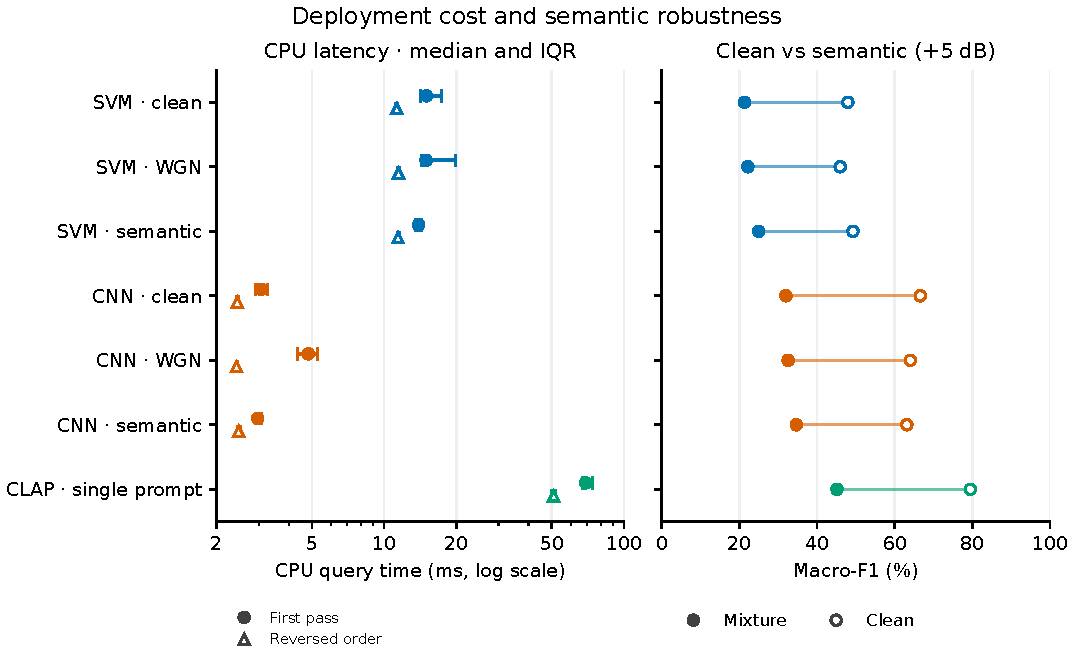
\includegraphics{../results/extensions_20261109/cost_figures/18_balanced_deployment_cost.pdf}
\caption{Balanced CPU latency alongside clean and +5-dB different-category macro-F1 under own-activity power. Both timing passes are retained; whiskers show each pass's interquartile range of 750 queries, not confidence intervals. CNN performance here uses seed 5305; the intervention analysis retains all three seeds.}
\end{figure}

External pretraining is excluded. CLAP
prompt embeddings are cached, and its audio embedding plus class scoring is
included. CPU performance is separate from MPS used for supervised training.
CLAP's reported preprocessing stage covers resampling and quantisation; its
internal Mel frontend is included in embedding time. Stage boundaries therefore
differ across implementations, so total query cost is the comparable measure.

The compact CNN has 36,258 parameters; the loaded CLAP model has 158,334,169.
Saved checkpoint size, parameter bytes and inference latency are different
quantities. CLAP's 1.86-GB checkpoint must not be compared to a small supervised
model file as though both contain identical kinds of state. The project measures
local deployment cost, not total lifetime training energy.

Power matching alone leaves spectral, temporal and perceptual differences uncontrolled.
The closing analysis measures several spectral and temporal proxies, but its
restricted matching does not eliminate the remaining acoustic or perceptual differences.
Only three DEMAND environments and one semantic pair of each category type per
target are sampled. Coarse ESC categories are not a direct measure of perceptual
similarity. At 0 dB either event may be a reasonable description. Frozen CLAP
has external pretraining advantages and potential dataset overlap. Source reuse,
post-baseline analysis choices and seed variability limit generalisation.
These limitations are reasons to report the protocol and failure cases precisely,
not reasons to reinterpret a smaller error bar as proof of causal semantics.

\section{Extension experiments}
\subsection{Protocol}
The extension compares clean, WGN-augmented and semantic-augmented supervised
training. CNN seeds are 5305, 5306 and 5307. Each augmented CNN sees clean data
with probability 0.5 and otherwise one of three fixed training-only views at
+5, +10 or +15 dB under the own-activity power convention. Both power conventions
are then evaluated at test time. Banks are shared across optimisation seeds. Clean validation,
architecture, training cap and four-fold refit logic are unchanged.
Actual refit epochs are selected separately on clean validation, so identical
augmentation probabilities and maximum budgets do not imply identical numbers
of training-example presentations. Semantic
partners come only from the current training partition; test DEMAND recordings
are never used for augmentation. The SVM uses equal counts of clean examples
and one balanced fixed augmented view per training clip. These interventions
test transfer from ordinary acoustic corruption to competing events.

A separate fixed prompt-ensemble ablation averages text embeddings over the
complete released PAT template list and reuses the exact cached CLAP audio
embeddings. It does not select prompts using labels and is not called full PAT.
The inspected reference implementation uses a different CLAP backend, local
features and a label-based fusion-coefficient search; reproducing that search
on outer test folds would invalidate this experiment's isolation. None of those
steps is silently incorporated into the core CLAP reference.

\subsection{Verified results}
The core and diagnostic results above are verified. The extended augmentation, multi-seed interference and prompt-ensemble results are still being generated and are not used to support the conclusions of this draft.
Completed additional clean training runs at the build time are seed 5306: clean accuracy 66.40\%, macro-F1 65.19\%; seed 5307: clean accuracy 66.40\%, macro-F1 65.53\%. Their interference comparisons are reported only after evaluation and audit.


\section{Completed scope and remaining limitations}
The declared extension is complete: three clean CNN seeds, WGN and semantic
training for SVM/CNN, fixed prompt ensembling, representation diagnostics and
balanced deployment timing. The prompt experiment uses the released PAT template
list, but does not implement PAT's full audio--text mutual alignment. Full PAT
and Mix-CLAP are therefore not reported as reproduced methods. The two closing
analyses---exact ranked-label readout and spectral--temporal overlap with DEMAND
completion---are also complete. Experimental work is closed at this scope;
no further models, datasets or training runs are proposed for this delivery.

Potential future studies, outside this project's completed scope, could reduce
identified uncertainties. First,
repeat held-out pairing with several fixed random seeds while keeping models
frozen; report variability across distractor choices rather than assuming one
pair per category type represents every competing scene. Second, construct and
validate spectrally and temporally matched interferer controls with reduced
recognisability. Recognisability must be checked rather than assumed from phase
randomisation or another transformation; residual acoustic changes would still
limit causal interpretation. Third, vary onset alignment for fixed source pairs
and use a denser SIR grid on a declared subset, checking event truncation and
achieved power after each shift. This would test overlap effects within pairs
and support transition-threshold estimates that three SIR points cannot provide.
The completed top-two diagnostic complements, but does not retrospectively
replace, the designated-target metric. A calibrated detector or a dataset with
exhaustive multi-event annotations would be a different evaluation task.

\section{Conclusion}
Interference power alone does not describe environmental-sound classifier
failure. The SVM is vulnerable to white-noise-induced feature change, while
CLAP shows substantial competing-event capture despite strong background-noise
performance. Both power protocols and matched overlap strata are needed to
interpret that pattern. The CNN contrast is directionally consistent across
three seeds in the high-overlap population; the original seed's corrected test
remains inconclusive. The smaller acoustic-closeness subsets do not reproduce
a negative CNN contrast, whereas CLAP retains a substantial negative contrast.
This population-dependent evidence rules out a simple explanation by nominal
power alone, without isolating semantics causally.

Training interventions reveal a practical trade-off. WGN augmentation strongly
protects the CNN against white noise but transfers little to semantic mixtures.
Semantic augmentation gives larger semantic point-estimate gains while reducing
clean CNN performance; its direct paired accuracy advantages over WGN training
remain uncertain after the declared correction. Prompt ensembling improves
CLAP's class readout without removing competing-event failures. Exact top-two
readout recovers the target rank in some original captures, but many mixtures
still exclude it from the returned pair. The project
therefore connects controlled DSP, representation diagnostics and deployment
cost with an explicit account of which robustness gains transfer and which do not.

\section*{Reproducibility and attribution}
The repository contains custom DSP, supervised baselines, deterministic mixers,
training/evaluation splits, score and embedding exports, analysis scripts and
figure data. LAION-CLAP, its checkpoint and the PAT prompt list are external
resources with explicit provenance. Model/data hashes and source snapshots
identify the executed versions. The original proposal is retained, and its power
definition change is documented above. AI-assisted implementation, checking and
draft preparation were used; the report and code remain subject to author
review and the course's disclosure requirements. All declared experimental runs
are complete and independently checked. Final recording and course submission
remain separate from these research outputs.

\clearpage
\begin{thebibliography}{12}
\raggedright
\bibitem{esc} K. J. Piczak, ``ESC: Dataset for Environmental Sound Classification,'' ACM Multimedia, 2015. \href{https://doi.org/10.1145/2733373.2806390}{doi:10.1145/2733373.2806390}.
\bibitem{esc_repo} K. J. Piczak, ESC-50 official dataset repository and documented caveats. \url{https://github.com/karolpiczak/ESC-50}.
\bibitem{piczak_cnn} K. J. Piczak, ``Environmental Sound Classification with Convolutional Neural Networks,'' MLSP, 2015. \href{https://doi.org/10.1109/MLSP.2015.7324337}{doi:10.1109/MLSP.2015.7324337}.
\bibitem{augmentation} J. Salamon and J. P. Bello, ``Deep Convolutional Neural Networks and Data Augmentation for Environmental Sound Classification,'' IEEE Signal Processing Letters, 2017. \href{https://arxiv.org/abs/1608.04363}{arXiv:1608.04363}.
\bibitem{demand} J. Thiemann et al., ``The Diverse Environments Multi-Channel Acoustic Noise Database (DEMAND),'' POMA, 2013. \href{https://doi.org/10.1121/1.4799597}{doi:10.1121/1.4799597}.
\bibitem{clap} Y. Wu et al., ``Large-Scale Contrastive Language-Audio Pretraining with Feature Fusion and Keyword-to-Caption Augmentation,'' ICASSP, 2023. \href{https://arxiv.org/abs/2211.06687}{arXiv:2211.06687}.
\bibitem{pat} A. Seth et al., ``PAT: Parameter-Free Audio-Text Aligner to Boost Zero-Shot Audio Classification,'' NAACL, 2025, pp. 12376--12394. \href{https://aclanthology.org/2025.naacl-long.616/}{doi:10.18653/v1/2025.naacl-long.616}.
\bibitem{mixclap} W. Kohno et al., ``Mix-CLAP: Adaptive Fusion of Knowledge-Distilled Audio Embeddings for Noise-Aware Audio-Language Models,'' ICASSP, 2026. \href{https://www.cmsworkshops.com/ICASSP2026/view_paper.php?PaperNum=4206}{Official conference record}.
\bibitem{rsa} Y. Zhang et al., ``RSA-Bench: Benchmarking Audio Large Models in Real-World Acoustic Scenarios,'' Findings of ACL, 2026, pp. 18350--18374. \href{https://aclanthology.org/2026.findings-acl.913/}{doi:10.18653/v1/2026.findings-acl.913}.
\bibitem{noncollapsibility} N. A. Schuster et al., ``Noncollapsibility and its role in quantifying confounding bias in logistic regression,'' BMC Medical Research Methodology, 2021. \href{https://doi.org/10.1186/s12874-021-01316-8}{doi:10.1186/s12874-021-01316-8}.
\end{thebibliography}

\clearpage
\appendix
\renewcommand{\corefig}[3]{\begin{figure}[htbp]\centering\includegraphics{../results/report_figure_assets_20261109/#1.pdf}\caption{#2}\label{#3}\end{figure}}
\section{Supplementary figures}
The following figures retain the original within-model scales and denominators.
The repository also contains a complete corresponding figure set for the target
power convention, each with numerical source tables and export audits.

\corefig{fig3_margin_vs_sir}{Target--distractor margin distributions. Scores have architecture-specific scales; comparisons are within each panel. A negative margin indicates a distractor score above the target score, not necessarily the overall predicted class.}{fig:margin}
\corefig{fig4_same_vs_different}{Same- versus different-category relative macro-F1 loss. Large markers are ratios of five-fold mean F1 values on common targets; small dots are the five individual fold ratios. A ratio of means is not generally the mean of ratios. Category relationships are coarse dataset groupings, not a validated perceptual-distance scale.}{fig:category}
\corefig{fig5_representation_displacement}{Representation displacement from gain-matched controls, separated by classification outcome. Handcrafted features use training-fold standardisation; CNN and CLAP use cosine distance. Absolute distances are not comparable between architectures.}{fig:representations}
\corefig{fig6_confusion_flow}{Observed target-to-distractor capture counts relative to available pairs. Counts include pre-existing clean-control confusions; they are not all newly induced errors. The source table separately counts captures from correct controls. Examples are selected by observed counts, and small denominators do not establish reliable class-pair risk.}{fig:flows}
\corefig{fig7_robustness_vs_cost}{Original own-protocol robustness and CPU microbenchmark at +5 dB different-category interference. The horizontal coordinate sums the median preprocessing and median inference times for one clip; it is not the median total over the balanced panel. Cached CLAP text embeddings are used; open markers show clean macro-F1. External pretraining cost is excluded.}{fig:cost}
\diagfig{12_displacement_error_association}{Association between representation displacement and classification error at +5 dB. Dots show the five official folds and short bars their means. AUC above 0.5 indicates larger movement tends to accompany errors; this is descriptive, not a causal semantic-effect estimate.}{fig:auc}
\corefig{fig8_overlap_strata}{Overlap-stratified semantic versus DEMAND comparisons on matched target sets. Read accuracy together with class coverage; macro-F1 with all 50 labels is sensitive to absent classes in small strata.}{fig:overlap}
\closingfig{21_capture_rank_retention}{Target inclusion among original argmax captures at +5 dB as the number of returned labels increases. Pointwise 95\% intervals resample original target-source clusters (2,000 replicates); repeated clips remain together. The target cannot be first in an argmax capture, so the $k=1$ value is zero by definition. Larger $k$ mechanically relaxes retrieval.}{fig:retention}
\closingfig{24_accuracy_by_masking}{Accuracy inside fixed time--frequency masking bins at +5 dB. Points and source-bootstrap intervals require at least 30 targets and source clusters. Condition groups inside a bin can contain different targets and classes; this display is descriptive, unlike the same-target comparisons in Figure~\ref{fig:acoustic-matched}. Empty or small bins are not interpolated.}{fig:masking-bins}
\end{document}
